% PDF 145
\sourcepage{141}{145}
结构层在每一点 $x\in X$（或 $y\in Y$）处的茎都是局部环。换句话说，(10.13) 也可以写为
\begin{equation}\tag{10.14}
 \Hom_{\G}(A,B)\hookrightarrow
 \Hom_{\mathsf{Lrs}}\bigl((X,\mathcal O_X),(Y,\mathcal O_Y)\bigr).
\end{equation}
不过，赋环空间的同态 $\varphi\colon X\to Y$ 意味着：每取一对满足 $y=\varphi(x)$ 的点 $x\in X$、$y\in Y$，就得到一个方向相反的环同态
\begin{equation}\tag{10.15}
 u_x\colon\mathcal O_{Y,y}\longrightarrow\mathcal O_{X,x},
\end{equation}
它连接 $y$、$x$ 两点处的茎。两个局部环之间的这个同态 $u_x$（它是 $\G$ 中的态射），只有在它是所谓\emph{局部同态}时才算是“合理”的；这就是说，极大理想 $\mathfrak m_x$ 的逆像恰好是极大理想 $\mathfrak m_y\subset\mathcal O_{Y,y}$，即
\begin{equation}\tag{10.16}
 u_x\text{ 是局部同态}\quad\Longleftrightarrow\quad
 u_x^{-1}(\mathfrak m_x)=\mathfrak m_y.
\end{equation}
\footnote{回忆：对局部环间任意同态 $u\colon\mathcal O\to\mathcal O'$，总有 $u^{-1}(\mathfrak m')\subset\mathfrak m$。当这一包含成为等式 $u^{-1}(\mathfrak m')=\mathfrak m$ 时，就称 $u$ 为局部同态；这等价于 $u(\mathfrak m)\subset\mathfrak m'$（参见前面的讨论，原文此处节号、页码空缺）。接着录音的内容说：这个条件保证 $u$ 可以下降到商，诱导剩余域之间的同态 $k\to k'$，其中 $k=\mathcal O/\mathfrak m$、$k'=\mathcal O'/\mathfrak m'$，使图
\[
\begin{tikzcd}[ampersand replacement=\&]
\mathcal O\arrow[r,"u"]\arrow[d,two heads]\&\mathcal O'\arrow[d,two heads]\\
k\arrow[r]\&k'
\end{tikzcd}
\]
交换，竖箭头是典范投影。另一种表述是 $f\in\mathcal O^*\Longleftrightarrow u(f)\in(\mathcal O')^*$。当然，不论两环是否局部，若 $f$ 可逆，则 $u(f)$ 也可逆；这里的反向蕴涵则由局部同态条件保证。}
\begin{center}
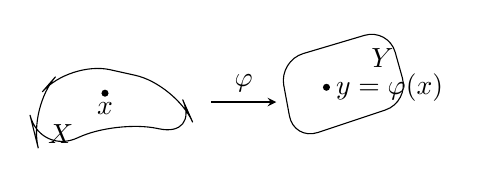
\begin{tikzpicture}[scale=.75,>=stealth]
\draw[rounded corners=15pt] (0,0) -- (-.2,.8) -- (.5,1.6) -- (2.3,1.2) -- (2.7,.3) -- (1.3,.6) -- cycle;
\node at (.35,.35) {$X$};\fill (1.1,1.05) circle (1.7pt);\node[below] at (1.1,1.05) {$x$};
\draw[->] (2.9,.9)--(4,.9) node[midway,above] {$\varphi$};
\draw[rounded corners=9pt] (4.3,.25)--(4.05,1.6)--(5.9,2.15)--(6.25,.9)--cycle;
\node at (5.8,1.65) {$Y$};\fill (4.85,1.15) circle (1.7pt);\node[right] at (4.85,1.15) {$y=\varphi(x)$};
\end{tikzpicture}
\end{center}
因此，赋环空间范畴 $\mathsf{Rs}$ 中的态射 $\varphi\colon(X,\mathcal O_X)\to(Y,\mathcal O_Y)$ 称为\emph{局部态射}，也称\emph{局部赋环空间的态射}（即 $\mathsf{Lrs}$ 中的态射），
% PDF 146
\sourcepage{142}{146}
当且仅当对每一对相应的点 $(x,\varphi(x))$，茎之间的同态 (10.15) 都是局部环的局部同态。现在可以证明，映射 (10.4) 中 $\Hom_{\G}(A,B)$ 的像由局部态射组成。反过来也成立，故 (10.4) 中的包含实际上是双射：
\begin{equation}\tag{10.16}
\begin{split}
\Hom_{\G}(A,B)&\xrightarrow{\sim}
\Hom_{\mathsf{Lrs}}\bigl((\Spec B,\widetilde B),(\Spec A,\widetilde A)\bigr)\\
&=\Mor_{\mathsf{Lrs}}(X,Y).
\end{split}
\end{equation}
\footnote{译注：原书在此重复使用了编号 (10.16)，本译本保留原编号。}
\Section{11}{找回失去的基环 $k$}
迄今建立的这部“字典”，把环与作为特殊局部赋环空间的仿射概形联系起来。它告诉我们，怎样用局部赋环空间 $(\Spec A,\widetilde A)$ 来解释 $\Ob\G$ 中的环 $A$；也可以说，解释反范畴中的对象 $\mathfrak X_A$，即我们从一开始就关心的仿射代数空间（参见第二章）。换言之，就是用与仿射代数空间 $\mathfrak X_A\in\Ob\Aff_{\mathbb Z}$ 一一对应的仿射概形来解释它。\footnote{$\Aff_{\mathbb Z}$ 表示绝对仿射代数空间的范畴，即 $\mathbb Z$ 上的仿射代数空间。稍后要用的范畴 $\Aff_k$ 则是 $k$ 上仿射代数空间的范畴，其中 $k\in\Ob\G$。}
用精确的范畴语言说，我们有函子
\begin{equation}\tag{11.1}
\mathsf{Sch}\colon\G\longrightarrow\mathsf{Lrs},\qquad
\mathsf{Sch}^{\circ}\colon\Aff_{\mathbb Z}\longrightarrow\mathsf{Lrs}.
\end{equation}
\footnote{这里已把 $\Aff_{\mathbb Z}$ 与 $\G$ 的反范畴 $\G^{\circ}$ 典范地等同。回忆 $\G=\G_{\mathbb Z}$（参见第一章第2节），即 $\G$ 中的环与 $\mathbb Z$-代数是一回事。}
$\mathsf{Sch}=(\Spec,\widetilde{\phantom A})$ 是反变函子，$\mathsf{Sch}^{\circ}$ 是协变函子。两者的像 $\mathsf{Sch}(\G)$、$\mathsf{Sch}^{\circ}(\Aff_{\mathbb Z})$ 都可以等同于
% PDF 147
\sourcepage{143}{147}
$\mathsf{Lrs}$ 的一个满子范畴。也就是说，$\mathsf{Sch}$ 与 $\mathsf{Sch}^{\circ}$ 都完全忠实（当然，$\mathsf{Sch}$ 要反转箭头）。
我们的基环 $k\in\Ob\G$ 似乎“失去”了，因为在构造 $\mathsf{Sch}(A)$ 时它没有起任何作用。现在需要看看怎样把它找回来。设
\begin{equation}\tag{11.2}
 u\colon k\longrightarrow A
\end{equation}
是 $k$-代数 $A$ 的结构态射。字典 (11.1) 给出两个映射：
\begin{equation}\tag{11.3}
\begin{gathered}
\mathsf{Sch}(u)\colon\mathsf{Sch}(A)\longrightarrow\mathsf{Sch}(k),\\
\mathsf{Sch}^{\circ}(\mathfrak X_k)\longrightarrow
\mathsf{Sch}^{\circ}(\mathfrak X_A).
\end{gathered}
\end{equation}
第一个反转箭头。\footnote{译注：第二个箭头的方向依原书保留；按 $\mathsf{Sch}^{\circ}$ 为协变函子以及 $\mathfrak X_A\to\mathfrak X_k$ 的对应关系，应为 $\mathsf{Sch}^{\circ}(\mathfrak X_A)\to\mathsf{Sch}^{\circ}(\mathfrak X_k)$。}
把 $\mathsf{Sch}(u)$ 分解为 $(\Spec u,\widetilde u)$，便看到 $\widetilde u\colon\widetilde k\to\widetilde A$ 给出了结构层之间的层同态。考察相应点处的茎，可得同态 $k\to\mathcal O_x\to\mathcal O_y$；取复合便知道，$\widetilde A$ 的每一个茎都由此获得了 $k$-代数结构。由于 $A\simeq\Gamma(X,\widetilde A)$，反过来也成立：$\widetilde A$ 上任意 $k$-代数层结构都给出 $A$ 的一个 $k$-代数结构态射 (11.2)。
这些讨论可概括如下。
重新把 $k\in\Ob\G$ 作为基环引入时，$\G$、$\mathsf{Lrs}$、$\Aff$、$\mathsf{Sch}$ 分别换成带下标 $k$ 的相应对象；特别有
\begin{equation}\tag{$11.1'$}
\mathsf{Sch}_k\colon\G_k\longrightarrow\mathsf{Lrs}_k,\qquad
\mathsf{Sch}^{\circ}_k\colon\Aff_k\longrightarrow\mathsf{Lrs}_k.
\end{equation}
这里 $\Aff_k$ 是 $k$ 上仿射代数空间的范畴，$\mathsf{Lrs}_k$ 是结构层 $\mathcal O_X$ 为 $k$-代数层的局部赋环空间范畴，等等。
% PDF 148
\sourcepage{144}{148}
取 $k=\mathbb Z$（即 $\G$ 的始对象，参见第一章第2节），便回到不显式提及 $k$ 的\emph{绝对情形}。
在经典代数几何中，$k$ 是域，而且常常是代数闭域；在早期探索的许多年间，人们取的都是 $k=\mathbb C$。这时 $(\Spec k,\widetilde k)$ 只由一个点 $(0)$ 及“附着”在该点上的域 $k$ 组成，即 $((0),k)$。此外，经典情形中的 $A$ 通常是有限生成 $k$-代数：$A=k[\xi_1,\xi_2,\ldots,\xi_n]$。
\Section{12}{仿射概形的例子；再论幂零元}
我们重新考察第5节原书第108页及以后各页的例子。现在已经知道，把 $\widetilde A$ 加到 $\Spec A$ 上，便可从局部赋环空间 $(\Spec A,\widetilde A)$ 恢复 $A$。在平凡情形 $(\Spec k,\widetilde k)$ 中我们已经看到这一点，那时底拓扑空间仅含一个点。
在来自不可约复代数簇 $V$ 的例子中，如果 $A$ 没有非零幂零元，那么“闭点” $\mathfrak m\in\Max A$ 处的茎就是局部环 $A_{\mathfrak m}$，其元素为“有理函数” $f/g$，其中 $f,g\in A$ 且 $g(\mathfrak m)\ne0$，即 $g\not\equiv0\pmod{\mathfrak m}$。非闭点 $\mathfrak p$ 处的茎则是如下有理函数的局部环：它们在 $\mathfrak p$ 所代表的不可约子簇 $W_{\mathfrak p}$ 上不取“$\infty$”值；换句话说，分母 $g(x)$ 在 $W_{\mathfrak p}$ 上不恒为零。
当 $V$ 不可约这一条件不成立时，就没有“有理函数域”。这再次显示了层论观点的优点：它取代旧有的双有理观点，而后者只适用于不可约簇。
$\widetilde{\mathbb Z}$ 在 $(0)\in\Spec\mathbb Z$ 处的茎是有理数域 $\mathbb Q$。此时 $\mathfrak m_0=0$，因而 $(0)$ 处的剩余域同构于 $\mathbb Q$。对任意素数 $p$，$\mathcal O_{X,(p)}$ 是由满足 $b\not\equiv0\pmod p$ 的有理数 $a/b$（$a,b\in\mathbb Z$）组成的环；$\mathfrak m_p$
% PDF 149
\sourcepage{145}{149}
是其中由 $a\equiv0\pmod p$ 的分数组成的理想，剩余域 $\kappa(p)$ 同构于特征为 $p$ 的素域 $\mathbb Z_p$。
给局部环 $\mathcal O$ 引入结构层，并无特别值得惊异之处。
\emph{$A$ 中是否有幂零元，并不影响结构层 $\widetilde A$ 的构造。}而 $A\simeq\Gamma(X,\widetilde A)$（$X=\Spec A$）表明：除非 $a=0$，否则 $a\in A$ 在所有 $\mathfrak p\in\Spec A$ 处的局部化不可能全为零。这说明，把 $\widetilde A$ 理解为局部函数芽所成的层，这种起初非常有用的解释，在一般情形下已不再适用。首先，值 $a(\mathfrak m_{\mathfrak p})\in\kappa(\mathfrak p)$ 所在的域随点变化；它不像经典的 $\Max A$ 情形那样，是固定的域 $k$。经典情形中，$A$ 是没有非零幂零元的有限生成 $k$-代数，且 $k$ 代数闭。如果误把 $\widetilde A$ 的全空间中的元素当作函数芽，那么对非零幂零元 $a\in A$ 就会得到这样的“悖论”：“函数本身非零，却在每一点 $x\in\Spec A$ 都取零值。”这恰好对应于
\[
 a\in\mathfrak p_x\quad(\forall x\in\Spec A)
 \quad\Longleftrightarrow\quad a\in\operatorname{Nil}A.
\]
\Section{13}{拟凝聚层与函子 $M\mapsto\widetilde M$}
我们研究协变函子
\[
 \widetilde{\phantom M}\colon\mathsf M_A\longrightarrow
 \operatorname{Mod}(\widetilde A),
\]
其中 $\mathsf M_A$ 是 $A$-模范畴，$\operatorname{Mod}(\widetilde A)$ 是 $X=\Spec A$ 上的 $\mathcal O_X$-模范畴，$\mathcal O_X=\widetilde A$。这是交换代数与赋环空间之间那部“字典”的一个极其重要的例子。
\textbf{Grothendieck 的概述。}我们要明确写出 $A$-模 $M\in\Ob\mathsf M_A$ 与环 $A$ 的谱 $X$ 上的 $\widetilde A$-模层 $\widetilde M$ 之间的函子性对应 $M\mapsto\widetilde M$。这里
\[
 X=\Spec A=\{\mathfrak p\mid\mathfrak p\text{ 是 }A\text{ 的素理想}\}
\]
视为拓扑空间，并配备环层 $\mathcal O_X=\widetilde A$（参见前文）。我们将看到，$A$-模范畴 $\mathsf M_A$ 可等同于 $X$ 上所有 $\widetilde A$-模所成范畴的一个满子范畴；这个子范畴恰好就是 $X$ 上所谓\emph{拟凝聚层}的范畴。对于任意赋环空间 $(X,\mathcal O_X)$，拟凝聚性都是 $\mathcal O_X$-模上的纯局部条件（参见第7节）：这些模在局部可以写成局部自由模之间同态的余核。
$A$-模与 $X$ 上模层之间的这部字典，几乎与我们能想到的各种构造都相容。具体说，这个函子与下列运算交换：
% PDF 150
\sourcepage{146}{150}
\begin{enumerate}[label=\arabic*)]
\item 有限和，即有限积；换句话说，函子 $M\mapsto\widetilde M$ 是加性的。
\item 张量积：
\begin{equation}\tag{13.1}
 \widetilde{M\otimes_A N}\xrightarrow{\sim}
 \widetilde M\otimes_{\widetilde A}\widetilde N.
\end{equation}
\item $\Hom$：
\begin{equation}\tag{13.2}
 \widetilde{\Hom_A(M,N)}\xrightarrow{\sim}
 \mathcal{H}om_{\widetilde A}(\widetilde M,\widetilde N),
\end{equation}
条件是第一个变量为有限表现模。此外：
\item 它是正合函子，即
\begin{equation}\tag{13.3}
\begin{gathered}
0\longrightarrow M'\longrightarrow M\longrightarrow M''\longrightarrow0
\quad\text{正合}\\
\Longrightarrow\quad
0\longrightarrow\widetilde M'\longrightarrow\widetilde M
\longrightarrow\widetilde M''\longrightarrow0
\quad\text{正合。}
\end{gathered}
\end{equation}
\item 它完全忠实。
\end{enumerate}
最后一点意味着，$\mathsf M_A$ 可视为 $\widetilde A$-模范畴 $\operatorname{Mod}(\widetilde A)$ 的一个满子范畴。
有一点值得特别强调：函子 $\widetilde{\phantom M}$ \emph{不与任意积交换}，即指标集 $I$ 不一定有限时，$\widetilde{\prod_{i\in I}M_i}$ 一般不与 $\prod_{i\in I}\widetilde M_i$ 典范同构：
\begin{equation}\tag{13.4}
 \widetilde{\prod_{i\in I}M_i}\not\simeq
 \prod_{i\in I}\widetilde M_i.
\end{equation}
事实上，只有在对每个 $f\in A$，同态
\[
 \left(\prod_{i\in I}M_i\right)_f\longrightarrow
 \prod_{i\in I}(M_i)_f
\]
都是同构时，上面否定的性质才会成立。\footnote{译注：原书此处把 (13.4) 误引作 (12.4)，下页也把 (13.2) 误引作 (12.2)。此处及下文按实际所指译出。}这当然不对！局部化不过是由 $A$ 到 $A_f$ 的换环的一个特例，而换环不与积交换。例如，令所有 $M_i$ 都等于 $A$，问题便成为 $(A^I)_f$ 是否自然同构于 $(A_f)^I$。看看这意味着什么：一边的元素是形如 $(\alpha_i/f^{n_i})_{i\in I}$ 的族，另一边则形如 $(x_i/f^n)_{i\in I}$，其中指数 $n$ 固定。显然，当 $I$ 无限时，指数 $n_i$
% PDF 151
\sourcepage{147}{151}
不必有上界！
同样还要小心，$\Hom(\ ,\ )$ 的形成一般也不与加波浪号的操作交换。也就是说，通常只有箭头
\[
 \widetilde{\Hom_A(M,N)}\longrightarrow
 \mathcal{H}om_{\mathcal O_X}(\widetilde M,\widetilde N),
\]
它一般不是同构。取 $M=A^I$ 且 $I$ 无限，便容易归结到前一种情况。正如上面第3点、公式 (13.2) 所说，适当的假设是 $M$ 为有限表现模。\footnote{译注：原书写作“第2点”，实际所指是第3点。原书写作 $M=A^I$，此处依原文保留；要直接归结到任意积不交换，通常取 $M=A^{(I)}$ 为无限直和。}
\Section{14}{集合层附录}
\footnote{本节笔记由 J. Winthrop 协助整理。}
下面关于集合层的笔记来自 Grothendieck 的拓扑斯课程开头几讲。若把它们放进第7节，就会离题太远，所以收入附录。我认为，这些内容既能帮助已读过 FAC 的读者，也可作为 Godement（戈德芒）那部经典著作\footnote{译注：原书把 Godement 误拼为 Codement。}所采用的抽象方法的入门。
我要讲拓扑斯理论。我喜欢把它看成经典一般拓扑学的一种推广。作为预备知识，我们假定大家熟悉拓扑空间、连续映射、同胚等等，另一方面也熟悉范畴语言。稍后我们会说明，为什么要引入比拓扑空间更一般的对象，并给出一些例子。不过，要理解拓扑斯理论，还需要熟悉拓扑空间上的层的语言。我想，并非人人都很熟悉这个概念，所以不预先假定大家已有这方面的知识。下面我将回顾拓扑空间上集合层的标准理论。\footnote{Grothendieck 主要讨论集合层，所以下文通常省去“集合”二字。不过他稍后也会引入各种代数结构。已经读过 FAC 的读者可以借这些讲义，将拓扑性质与代数性质区分开来，从而加深对层论的理解。}
% PDF 152
\sourcepage{148}{152}
\subsection*{14.-1.\quad 集合预层}
设 $X$ 是拓扑空间。考虑 $X$ 的开子集所成的集合 $\mathcal O=\operatorname{Op}(X)$；它是幂集 $\mathfrak P(X)$ 的一个子集，并确定 $X$ 上的拓扑。\footnote{记号来自法语 partie，即子集；$\mathfrak P(X)=2^X$。}回忆拓扑公理：$\operatorname{Op}(X)$ 包含 $\varnothing$ 和 $X$ 本身，且对任意并与有限交封闭。$\operatorname{Op}(X)$ 按包含关系构成偏序集，因此稍稍滥用语言，也就构成了范畴。这个范畴仍记为 $\mathcal O$ 或 $\operatorname{Op}(X)$。同一般偏序集 $C$ 一样，对对象 $U,V\in C$，从 $U$ 到 $V$ 的“同态”集合 $\Hom(U,V)$，在 $U$ 不包含于 $V$ 时为空；否则只含 $U$ 到 $V$ 的“包含映射” $i\colon U\hookrightarrow V$：
\begin{equation}\tag{1.1}
 \Hom(U,V)=\begin{cases}
 \varnothing,&U\nsubseteq V,\\
 \{i\colon U\hookrightarrow V\},&U\subseteq V.
 \end{cases}
\end{equation}
箭头 $U\to V\to W$ 的复合按显然的方式定义，事实上也没有别的选择。这种范畴构造对任意偏序集 $C$ 都有意义，并未用到 $C=\operatorname{Op}(X)$ 这一事实。
换言之，范畴 $\operatorname{Op}(X)$ 的对象是 $X$ 的开集，箭头则由包含关系的图给出。\footnote{一般地，序集 $(S,<)$ 所对应的范畴，其箭头由关系图 $\operatorname{Graph}(<)=\{(x,y)\in S\times S\mid x<y\}$ 给出。这里 $S=\operatorname{Op}(X)$，而序关系 $<$ 是包含关系 $\subseteq$。}
按定义，$X$ 上的\emph{预层} $F$ 是从 $\operatorname{Op}(X)$ 到集合范畴的反变函子。换句话说，$F$ 是从 $\operatorname{Op}(X)$ 的反范畴 $\mathcal O^{\circ}$ 到集合范畴 $\Sets$ 的函子。
回忆这意味着什么。
\begin{enumerate}[label=\arabic*)]
\item 对范畴的每一个对象，即 $X$ 的每一个开集 $U$，指定一个集合 $F(U)$，其元素称为 $F$ 在 $U$ 上的截面。
\end{enumerate}
% PDF 153
\sourcepage{149}{153}
\footnote{“截面”这一术语来自过去用平展覆盖空间 $p\colon S\to X$ 直接定义 $X$ 上的层的方法（参见后面一小节）。若 $U$ 是 $X$ 的开集，则 $U$ 上的截面是满足 $p\circ s=1_U$ 的映射 $s\colon U\to S$。}
\begin{enumerate}[label=\arabic*),start=2]
\item 对每个包含映射 $i\colon U\hookrightarrow V$，指定相应集合间的反向映射
\begin{equation}\tag{1.2}
 \rho_V^U\colon F(V)\longrightarrow F(U).
\end{equation}
这里 $\rho_V^U=F(i)$，也用限制记号表示：
\begin{equation}\tag{1.3}
 F(V)\longrightarrow F(V)|_U=\rho_V^U(F(V)).
\end{equation}
\end{enumerate}
还须满足以下“显然的”公理。
\textbf{传递性。}若另一个开集 $W$ 包含 $V$，即有 $X$ 中开集的包含 $U\hookrightarrow V\hookrightarrow W$，那么集合范畴中的箭头 $F(W)\to F(V)\to F(U)$ 保持复合。也就是说，下面左边的交换图对应于右边的交换图：
\begin{equation}\tag{1.4}
\begin{tikzcd}[ampersand replacement=\&]
U\arrow[r,hook]\arrow[dr,hook]\&V\arrow[d,hook]\\
\&W
\end{tikzcd}
\qquad\longmapsto\qquad
\begin{tikzcd}[ampersand replacement=\&]
F(U)\&F(V)\arrow[l]\\
\&F(W)\arrow[u]\arrow[ul]
\end{tikzcd}
\end{equation}
\textbf{恒等性。}$F$ 将恒等映射变成恒等映射：$U\xrightarrow{\id}U$ 对应于 $F(U)$ 到自身的恒等映射 $F(U)\to F(U)$。
$X$ 上的预层范畴
\[
 \operatorname{Presh}(X)=\Hom(\mathcal O^{\circ},\Sets)
\]
定义为所有函子 $\mathcal O^{\circ}\to\Sets$ 构成的范畴。也就是说，$\operatorname{Presh}(X)$ 的对象就是函子 $F\colon\mathcal O^{\circ}\to\Sets$。
按函子同态的定义，$X$ 上两个预层 $F$、$G$ 之间的同态 $f\colon F\to G$\footnote{Grothendieck 较喜欢“函子同态”这个说法，而不用范畴论中很常见的同义术语“自然变换”。}，就是一族
% PDF 154
\sourcepage{150}{154}
与限制映射相容的映射 $F(U)\to G(U)$（$U\in\Ob\mathcal O(X)$）。亦即，对每一个 $X$ 的开集 $U$，有映射 $f(U)\colon F(U)\to G(U)$，使下图交换：
\begin{equation}\tag{1.6}
\begin{tikzcd}[ampersand replacement=\&]
F(U)\arrow[r,"f(U)"]\&G(U)\\
F(V)\arrow[u]\arrow[r,"f(V)"']\&G(V)\arrow[u]
\end{tikzcd}
\end{equation}
竖箭头是对应于 $U\subseteq V$ 的限制映射。此外，预层态射 $F\xrightarrow fG\xrightarrow gH$ 的复合，显然可由下图定义，其中各方块都交换：
\begin{equation}\tag{1.7}
\begin{tikzcd}[ampersand replacement=\&]
F(U)\arrow[r,"f(U)"]\&G(U)\arrow[r,"g(U)"]\&H(U)\\
F(V)\arrow[u]\arrow[r,"f(V)"']\&G(V)\arrow[u]\arrow[r,"g(V)"']\&H(V)\arrow[u]
\end{tikzcd}
\end{equation}
构造范畴 $\operatorname{Presh}(X)$ 所需的那一点“一般废话”就是这些。到现在为止，我们尚未用到开集范畴 $\mathcal O(X)$ 的性质，只用了函子态射，也就是“自然变换”的性质。现在则要利用前者，定义一类特殊的预层：$X$ 上的层。
\subsection*{14.-2.\quad 集合层}
我们要在预层上引入刻画层的公理。这些公理可用两个性质来表达。
设 $F$ 是 $X$ 上的预层。对 $X$ 的每个开集 $U$ 及其每个开覆盖 $(U_i)_{i\in I}$，即 $U=\bigcup_{i\in I}U_i$，考虑从 $F(U)$ 到各个 $F(U_i)$ 的限制映射，于是得到到它们的积的映射
\begin{equation}\tag{2.1}
 F(U)\longrightarrow\prod_{i\in I}F(U_i).
\end{equation}
\footnote{并集也可以用 $\operatorname{Op}(X)$ 中的偏序来定义：$U$ 是全部 $U_i$（$i\in I$）的上确界。}
% PDF 155
\sourcepage{151}{155}
若对 $U$ 及其覆盖 $(U_i)_{i\in I}$ 的任意选择，上述映射 $F(U)\to\prod_{i\in I}F(U_i)$ 都是单射，就称 $F$ \emph{分离}。
换一种说法：预层 $F$ 赋予每个开集 $U\subseteq X$ 的集合，称为 $F$ 在 $U$ 上的截面集合；\footnote{这个术语来自用平展覆盖空间 $p\colon S\to X$ 直接定义层的旧方法（参见后面一小节）。当 $U$ 开时，$U$ 上的截面是满足 $p\circ s=1_U$ 的映射 $s\colon U\to S$。}对每个包含 $U\hookrightarrow V$，限制映射 $F(V)\to F(U)$ 给出限制后的截面。那么，预层 $F$ 分离，意味着：对 $U\in\Ob\operatorname{Op}(X)$ 的任意开覆盖 $(U_i)_{i\in I}$，一个 $U$ 上的截面由它在所有 $U_i$ 上的限制完全确定。即 (2.1) 的箭头是单射，所以可改写为
\begin{equation}\tag{2.2}
 F(U)\hookrightarrow\prod_{i\in I}F(U_i).
\end{equation}
用文字说，$F$ 在 $U$ 上的每个截面，都可等同于它在各个 $U_i$ 上的限制组成的截面族。
为把层刻画成特殊的预层，还需问第二个问题：任给一族截面 $\varphi_i\in F(U_i)$，能否把它们看成某个 $U=\bigcup_{i\in I}U_i$ 上的截面的限制？这样的截面存在的必要条件是“匹配性质”：对每对 $(i,j)\in I\times I$，有
\begin{equation}\tag{2.3}
 \varphi_i|_{U_i\cap U_j}=\varphi_j|_{U_i\cap U_j}.
\end{equation}
由限制映射的传递性可知，这个条件显然必要。
% PDF 156
\sourcepage{152}{156}
\textbf{定义 1.1。}称 $X$ 上的预层 $F$ 为\emph{层}，如果对每个 $U\in\Ob\mathcal O(X)$ 及 $U$ 的每个开覆盖，映射 (2.1) 不仅是单射（即 $F$ 分离），而且其像恰好由 $\prod_jF(U_j)$ 中满足 (2.3) 的所有元素组成；此处 (2.3) 须对每一对 $(i,j)\in I\times I$ 成立。
定义1.1也可以用图表语言写成：下列序列正合，
\begin{equation}\tag{2.4}
 F(U)\hookrightarrow\prod_{i\in I}F(U_i)
 \rightrightarrows\prod_{(i,j)\in I\times I}F(U_i\cap U_j).
\end{equation}
为解释 (2.4)，把 $F$ 作用于两个包含映射 $U_i\cap U_j\hookrightarrow U_i$ 与 $U_i\cap U_j\hookrightarrow U_j$。于是有两个限制箭头：$F(U_i)\to F(U_i)|_{U_i\cap U_j}$ 和 $F(U_j)\to F(U_j)|_{U_i\cap U_j}$。双箭头的“核”是 $\prod_{i\in I}F(U_i)$ 中那些截面族，它们对每一对 $(i,j)$，沿这两个限制映射所得的结果相同。因此 (2.3) 表达的恰好是正合性的通常含义，即像等于核。
对于两个层 $F$、$G$，\emph{层态射} $F\to G$ 按定义就是它们之间的预层态射。这样便得到范畴 $\operatorname{Top}(X)$，即 $X$ 上的层范畴；它是 $X$ 上预层范畴 $\operatorname{Presh}(X)$ 的满子范畴：
\begin{equation}\tag{2.5}
 \operatorname{Top}(X)\hookrightarrow\operatorname{Presh}(X)
 =\Hom(\mathcal O^{\circ},\Sets).
\end{equation}
现在该给出例子了，以说明层是一个很自然的概念，而且在数学中出现得十分频繁。
% PDF 157
\sourcepage{153}{157}
\textbf{例。}设 $E$ 是任意集合，在 $X$ 上定义预层 $F$：
\begin{equation}\tag{2.6}
 F(U)=\operatorname{Map}(U,E)=E^U,
 \qquad U\in\Ob\operatorname{Op}(X).
\end{equation}
即 $F(U)$ 是所有从 $U$ 到 $E$ 的映射组成的集合。
若有 $U\hookrightarrow V$，则把 $V$ 到 $E$ 的映射限制到 $U$ 上，便定义了 $F(V)=\operatorname{Map}(V,E)$ 到 $F(U)$ 的限制映射。也就是说，若 $\varphi\colon V\to E$ 属于 $\operatorname{Map}(V,E)$，则 $\varphi|_U\colon U\to E$ 属于 $\operatorname{Map}(U,E)$。由于映射的限制满足传递性，这确实定义了一个预层。
由 (2.6) 定义的预层 $F$ 实际上是层：若 $X$ 中的开集 $U$ 被一族 $U_i$（$i\in I$）覆盖，那么给定从 $U$ 到 $E$ 的映射，等价于给定各个 $U_i$ 到 $E$ 的映射，且这些映射对每对 $(i,j)\in I\times I$ 都在 $U_i\cap U_j$ 上“匹配”。事实上，即使 $U_i$ 不在 $X$ 中开，这仍然成立。
这样得到的层称为\emph{从 $X$ 到 $E$ 的映射层}。
数学中许多自然出现的层，都是这个层的子层。不过，在说明这一点以前，先要定义子预层和子层。
设 $F$、$G$ 都是 $X$ 上的预层。称 $G$ 为 $F$ 的\emph{子预层}，记作 $G\hookrightarrow F$，当且仅当下列两个条件成立：
\begin{enumerate}[label=\alph*)]
\item 对每个开集 $U\subseteq X$，$G(U)\hookrightarrow F(U)$，即 $G(U)$ 是 $F(U)$ 的子集。
\end{enumerate}
% PDF 158
\sourcepage{154}{158}
\begin{enumerate}[label=\alph*),start=2]
\item 对开集间的每个包含 $U\hookrightarrow V$，限制映射 $G(V)\to G(U)$ 由 $F(V)\to F(U)$ 诱导，即有显然的交换图。
\end{enumerate}
这正是一般所说的给定函子的子函子。
换言之，$G$ 是 $F$ 的子预层，当且仅当它由一族子集 $G(U)\subseteq F(U)$ 给出，而对这族子集所需的唯一条件，就是它在限制映射下封闭。
现在假定 $F$、$G$ 都是 $X$ 上的层。$G$ 是 $F$ 的\emph{子层}，当且仅当 $G$ 是 $F$ 的子预层。因此，$F$ 的子层由 $F(U)$ 的子集 $G(U)$ 组成；按预层的规则，这族子集须在限制映射下封闭。但现在还须保证预层 $G$ 本身是层，因而需要附加条件。
显然，若 $G$ 是层 $F$ 的子预层，则 $G$ 分离。因为，如前所述，若开集 $U$ 被开集 $U_i$（$i\in I$）覆盖，那么给定在各 $G(U_i)$ 中的截面，也就给定了它们在各 $F(U_i)$ 中的像；由于 $F$ 是层，这些像唯一确定可能的 $F(U)$ 中的截面，而 $G(U)\subseteq F(U)$ 又保证了 $G(U)$ 中截面的唯一性。
我们实际上刚刚证明：分离预层的子预层仍分离。那么，$G$ 不仅分离，而且还是层，意味着什么？这意味着赋值 $U\mapsto G(U)$ 具有局部性质。\footnote{称 $X$ 的开集所具有的性质 $P$ 为局部性质，是指对任意开集 $U$ 及其任意开覆盖 $(U_i)_{i\in I}$，只要每个 $U_i$ 上都具有性质 $P$，$U$ 上就具有性质 $P$。原书此处将后一个 $U$ 写成 $X$，按上下文译出。}概括起来：$X$ 上层 $F$ 的子层 $G$，由一族与限制映射相容的子集 $G(U)\subseteq F(U)$（$U\in\Ob\mathcal O(X)$）定义，并且“一个截面属于 $G(U)$”是局部性质。
% PDF 159
\sourcepage{155}{159}
\textbf{例。}假定前面的集合 $E$ 是拓扑空间，对每个 $U$，考虑从 $U$ 到 $E$ 的连续映射集合 $\operatorname{Cont}(U,E)$。\footnote{原文注：若给 $E$ 赋予离散拓扑，这一情形包含前面的 $\operatorname{Map}(U,E)$ 情形。译注：这里若要得到全部映射，应给 $E$ 赋予不可分拓扑，即只有空集与全集为开集的拓扑；离散拓扑对应的则是局部常值映射。}原文此处还写道，复合 $p\circ s$ 是 $U$ 到 $X$ 的包含映射。\footnote{译注：这一句涉及的 $p$、$s$ 在本例尚未定义，其含义见下一页关于纤维空间局部截面的例子。}
于是 $\operatorname{Cont}(U,E)\subseteq\operatorname{Map}(U,E)$，并且这一条件与限制映射相容，因为连续映射的限制仍连续。此外，我们知道连续性是局部性质：映射 $f\colon U\to E$ 连续，当且仅当对覆盖 $U$ 的开集族 $(U_i)$，所有限制 $f|_{U_i}$ 都连续。因此我们定义了从 $X$ 到 $E$ 的映射层的一个子层，即\emph{局部连续映射 $U\to E$ 所成的层}。
再例如，设 $X$ 是微分流形，其可微类别固定为 $C^r$（$r\ge1$）或 $C^{\infty}$，$E$ 也是同一类别的微分流形。考虑局部可微映射的集合 $\operatorname{Diff}(U,E)$，就得到上述局部连续映射层的一个子层。\footnote{即局部函数芽所成的层，其中局部函数可要求连续、$C^n$、$n\ge1$ 次可微、解析，等等。}众所周知，可微性是纯局部的性质，且在限制下保持。若 $U$ 被开集 $U_i$ 覆盖，那么 $f\colon U\to E$ 是 $C^r$ 映射，当且仅当每个 $f|_{U_i}\colon U_i\to E$ 都是 $C^r$ 映射；对 $U$ 的任意开覆盖 $(U_i)_{i\in I}$ 都是如此。
\textbf{3)} 这一做法还可任意推广，例如把微分流形换成解析簇、代数簇等等。因此，每一种“簇”都相应地定义了一类层。
\textbf{4)} 还有另一类子层的例子，可用纤维空间来描述。
% PDF 160
\sourcepage{156}{160}
设 $E$ 是 $X$ 上的纤维空间；也就是说，$E$、$X$ 是拓扑空间，并给定连续映射 $p\colon E\to X$。\footnote{不假定 $p$ 为满射。}三元组 $(E,X,p)$ 是一般的连续纤维空间，其中 $X$ 为底空间，$E$ 为全空间，$p$ 为投影。
对 $X$ 的每个开子集 $U$，考虑所有满足 $p\circ s=1_U$ 的连续映射 $s\colon U\to E$ 所成的集合 $\Gamma(U,E/X)$。这样的 $s$ 通常称为 $E$ 在 $U$ 上的\emph{截面}；若不想指明 $U$，则简称\emph{局部截面}。每个包含 $U\hookrightarrow V$ 都诱导映射 $\Gamma(V,E/X)\to\Gamma(U,E/X)$，即限制映射把 $V$ 上的截面变成 $U$ 上的截面。
现在很清楚，映射 $s\colon U\to E$ 是 $U$ 上的连续截面，当且仅当对 $U$ 的任意开覆盖 $(U_i)$，所有限制 $s|_{U_i}\to E$ 都是 $U_i$ 上的连续截面。这个层称为\emph{纤维空间 $p\colon E\to X$ 的局部截面层}。正是由于这个特殊例子，才引入了“$F$ 在 $U$ 上的截面”这一名称。
听众还有别的例子吗？
Schanuel 建议指出，前一个例子可以从本例，即纤维空间的局部连续截面层，取乘积 $E\times X$ 而得到。Grothendieck 表示同意。
若给 $E$ 赋予离散拓扑，并给 $X\times E$ 赋予积拓扑，那么前面的层也可以解释为 $X\times E\xrightarrow pX$ 的局部截面层，这里的 $p$ 是到第一个因子的投影。这时截面 $s\colon U\to X\times E$ 可以等同于函数 $f\colon U\to E$，对应关系为 $x\mapsto(x,f(x))$，而且这一对应与限制映射相容。\footnote{译注：原文末式写作 $x\mapsto(x,f(e))$，其中 $e$ 应为 $x$。这里若 $E$ 为离散空间，所得层就是到 $E$ 的局部常值函数层。}
% PDF 161
\sourcepage{157}{161}
还有其他例子吗？……再举几个吧。
设 $X$ 是局部紧拓扑空间。给它的每个开集 $U$ 指定 $U$ 上的 Radon 测度集合，这一赋值与限制映射相容。又由于这个性质是局部的，我们得到一个层，即局部紧空间 $X$ 的开集上的 Radon 测度层。
若 $X$ 是微分流形，可以考虑 $X$ 上的分布层：分布是 $X$ 上局部函数向量空间上的连续线性泛函，等等。分布可以局部化，因此又得到一个层。
另一个例子是：给 $X$ 的每个开集 $U$ 指定 $U$ 中相对闭的子集所成的集合。限制映射满足传递性，于是得到预层。这个预层是层，因为 $C\subseteq U$ 在 $U$ 中闭，当且仅当对 $U$ 的任意开覆盖 $(U_i)$，$C\cap U_i$ 在每个 $U_i$ 中都闭。也就是说，闭性是局部性质。
一般地，开集的子集所具有的任何局部性质，都可以用来定义 $X$ 上的层。例如，若 $X$ 是解析簇，就可以定义 $X$ 的局部解析子集所成的层。
一般说来，层是把局部信息转化为整体信息的最系统的工具，也就是说，层使我们能够把局部资料“综合”为整体性质。
现在设 $\mathcal E=(E,X,p)$ 是 $X$ 上的纤维空间，也简称为 $\mathcal E$。我们给 $E$ 指定一个层 $\widetilde E$，称为 $E$ 的局部连续截面层。
% PDF 162
\sourcepage{158}{162}
给 $X$ 上每个纤维空间 $E$ 指定层 $\widetilde E$，就得到函子性对应 $E\mapsto\widetilde E$。换言之，若有 $X$ 上纤维空间的态射 $f\colon E\to F$，即使下列三角形交换的全空间之间的连续映射，
\[
\begin{tikzcd}[ampersand replacement=\&]
E\arrow[rr,"f"]\arrow[dr,"p"']\&\&F\arrow[dl,"p"]\\
\&X\&
\end{tikzcd}
\]
便可定义态射 $\widetilde E\to\widetilde F$。事实上，给定 $X$ 的开集 $U$ 上的截面 $s\colon U\to E$，复合 $f\circ s$ 就是同一 $U$ 上 $F$ 的截面。映射 $s\mapsto f\circ s$ 与限制映射相容，故得到层同态 $\widetilde f\colon\widetilde E\to\widetilde F$。当 $f$ 变化时，对应 $f\mapsto\widetilde f$ 还与 $X$ 上纤维空间映射的复合相容，于是得到函子
\begin{equation}\tag{1.3}
 \operatorname{Fib}(X)\longrightarrow\operatorname{Top}(X),
\end{equation}
从 $X$ 上纤维空间范畴 $\operatorname{Fib}(X)$ 到 $X$ 上层范畴 $\operatorname{Top}(X)$。
首先自然会问：只知道 $\operatorname{Fib}(X)$ 中某个对象在 $\operatorname{Top}(X)$ 中的像，能否把这个对象重建出来？也就是说，能否由对应的层 $\widetilde E$ 重建 $X$ 上的纤维空间 $\mathcal E$？用形式语言说，我们想知道函子 (1.3) 是否完全忠实。
答案是否定的，而且很容易看出来。考虑特殊情形 $X=\{e\}$，即 $X$ 只有一个点 $e$。单点空间上的纤维空间范畴恰好等价于拓扑空间范畴，因为对每个拓扑空间 $E$，只有一个映射 $E\to\{e\}$。
% PDF 163
\sourcepage{159}{163}
因此 $\operatorname{Fib}(e)\simeq\mathfrak T$，其中 $\mathfrak T$ 是所有拓扑空间的范畴。另一方面，单点空间 $\{e\}$ 上的层范畴 $\operatorname{Top}(\{e\})$ 是什么？仍考察给 $\{e\}$ 指定截面 $\{e\}\to E$ 的映射。在典范等价意义下，单点空间上的层由相应的集合 $E$ 完全确定。因此，当 $X=\{e\}$ 时，函子 (1.3) 化为从所有拓扑空间范畴到集合范畴的函子 $\mathfrak T\to\Sets$，它把拓扑空间 $E$ 送到它的底抽象集合。也就是说，这是一个遗忘函子，只是把 $E$ 上的拓扑“忘掉”了！显然，这个函子不是完全忠实的：不能由底集合恢复 $E$ 的拓扑。因此，给定 $X$ 上的纤维空间 $\mathcal E$，比给定其局部连续截面层 $\widetilde E$，包含多得多的信息！
\subsection*{14.-3.\quad $X$ 的平展覆盖范畴 $\operatorname{\text{Ét}}(X)$}
现在可以问，能否在 $X$ 上纤维空间范畴 $\operatorname{Fib}(X)$ 中定义一个满子范畴 $\operatorname{\text{Ét}}(X)$，使函子 (1.3) 限制到它以后成为完全忠实函子？例如，在单点空间 $\{e\}$ 的情形，哪些拓扑空间的拓扑能由相应的底集合确定呢？有多种选择。其中一种是赋予离散拓扑：对给定集合 $S$，其上的离散拓扑只有一个。因此，若把函子 (1.3) 限制到 $\{e\}$ 上的离散拓扑空间范畴，就得到范畴等价。
我们希望把这个范畴等价推广到任意底空间 $X$。所以要定义 $\operatorname{Fib}(X)$ 的一个满子范畴，
% PDF 164
\sourcepage{160}{164}
使它在 $X=\{e\}$ 时退化为 $\{e\}$ 上的离散拓扑空间范畴。这样看来，适当的性质就是拓扑空间 $E$ \emph{在 $X$ 上平展}。现在来定义它！
拓扑空间之间的连续映射 $\pi\colon E\to X$ 称为\emph{平展映射}，如果它是局部同构，确切地说：对每个点 $x\in E$，存在 $x$ 的开邻域 $V\subseteq E$，使得 $\pi(V)$ 在 $X$ 中开，且 $\pi$ 诱导的映射 $V\to\pi(V)$ 是同胚。这就是说，$\pi$ 看起来像是上层空间 $E$ 中若干开集与它们在下层的投影 $\pi(V)$ 之间的一族局部同胚。
这时也称 $\pi$ 为拓扑空间 $E$、$X$ 之间的\emph{平展态射}。事实上，这个概念在单复变函数论中已有悠久历史，那里会出现一些在复平面的开子集上平展的映射。
下面举几个“平展性”的例子。
最明显的是开集 $U$ 到 $X$ 的包含映射 $U\hookrightarrow X$，这就是标准模型！
另一个例子：取离散拓扑空间 $I$，即给抽象集合 $I$ 赋予离散拓扑，并考虑积空间 $E=I\times X$。这意味着取各个副本 $\{a\}\times X$（$a\in I$）的不交和；每个副本都在 $E$ 中开。投影 $I\times X\to X$ 限制到这些 $X$ 的开副本上，就是“恒等映射” $(a,x)\mapsto x$。
现在构造 $X$ 的平展覆盖空间范畴 $\operatorname{\text{Ét}}(X)$，它是 $\operatorname{Fib}(X)$ 的子范畴。考察从 $\operatorname{Fib}(X)$ 到 $X$ 上层范畴 $\operatorname{Top}(X)$ 的函子 (1.3)，
% PDF 165
\sourcepage{161}{165}
把它限制到子范畴 $\operatorname{\text{Ét}}(X)$。这样便得到我们所寻求的、单点空间上的离散空间情形的推广！我们得到范畴等价
\begin{equation}\tag{3.1}
 \operatorname{\text{Ét}}(X)\xrightarrow{\sim}\operatorname{Top}(X).
\end{equation}
因此，可以把层本身，或 $X$ 的平展覆盖空间，即 $\operatorname{\text{Ét}}(X)$ 的对象，作为研究对象，并在这两种语言间来回转换。对层所作的某些运算，截面语言最方便；另一些运算则用平展空间的语言更好。
\textbf{例。}现在也许该再给几个例子。大家有什么建议吗？
\textbf{问：}法语形容词 \emph{étale} 没有英语译词吗？
\textbf{答：}没有。大约十五年前就有人问过这个问题。法语里说 \emph{un espace étalé dans un autre}，意思是一个空间“铺展在另一个空间上”。但谈态射时，说它是“铺展开的”听起来不太合适。那么，为什么不给英语引进一个新词呢？
Duskin 问，为什么不直接说“局部同胚”？Grothendieck 回答说，在微分空间、解析空间或代数空间的类似语境中，我们希望使用同一个词，因为形式性质是相同的，而不必分别引入局部微分同胚、局部双全纯映射等说法。最好有一个词适用于所有这些特殊情形。\footnote{后来私下交谈时，Grothendieck 告诉我，即使在他的母语德语中，也直接使用 étale 这个词，而不另找译词。}
\textbf{问：}最早的平展映射例子，是不是来自用复平面的若干副本构造 Riemann 曲面？
\textbf{答：}是的，只要把分支点去掉！好，就举这个例子：考虑仿射复直线到自身的映射
\[
 f\colon\mathbb C\longrightarrow\mathbb C,
 \qquad x\longmapsto x^n\quad(n\ge2).
\]
有 $f(0)=0$。把它限制为 $\mathbb C^*\to\mathbb C^*$，其中 $\mathbb C^*=\mathbb C\setminus\{0\}$，就得到平展映射。事实上，第二个复平面中非零点 $x$ 上的纤维，就是
% PDF 166
\sourcepage{162}{166}
$x$ 的 $n$ 个 $n$ 次根 $x_1,x_2,\ldots,x_n$ 所成的集合。选定其中一个，其余便可通过乘以 $n$ 次单位根得到，这些单位根为
\[
 \exp(2\pi\mathrm i h/n),\qquad h=0,1,\ldots,n-1.
\]
\footnote{译注：原文指数中写 $k$，后面列举指标时写 $h$；这里统一为 $h$。}
于是，对 $x$ 的不含 $0$ 的开邻域 $U$，便得到 $U$ 的 $n$ 个副本，每个都同胚地覆盖 $U$。\footnote{译注：这里需把 $U$ 取为充分小的邻域，例如不含 $0$ 的小圆盘。仅假定 $0\notin U$，一般不足以保证覆盖在整个 $U$ 上分裂为 $n$ 个副本。}由此看到，$x$ 是否为零，决定了映射的不同表现。把映射限制在零点的邻域时，它并不平展，$0$ 是一个分歧点。
\textbf{2)} 前一个例子可推广到两条不可约非奇异复曲线之间任意支配态射 $f\colon X\to Y$，即 $f(X)$ 在 $Y$ 中稠密的态射。去掉 $Y$ 中有限多个点，即分歧值 $R$，并把 $f$ 限制到
\[
 X\setminus\bigcup_R f^{-1}(R),
\]
就得到平展映射。
\textbf{3)} 第三个处处平展的覆盖例子，是连通拓扑流形 $X$ 的万有覆盖空间到它的覆盖映射 $\widehat X\to X$。
